\documentclass[border=10pt]{standalone}
\usepackage{tikz}
\usetikzlibrary{automata, positioning, arrows.meta}

\begin{document}
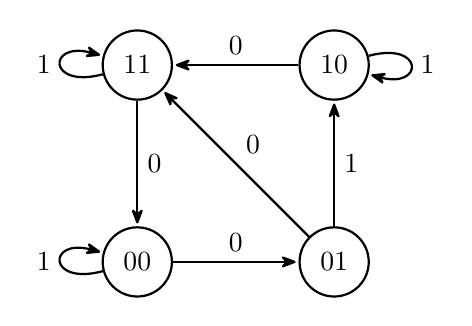
\begin{tikzpicture}[shorten >=1pt, node distance=2.5cm, on grid, auto, >={Stealth[round]}, thick]
    % Nodes
    \node[state] (s00) {00};
    \node[state] (s01) [right=of s00] {01};
    \node[state] (s11) [above=of s00] {11};
    \node[state] (s10) [right=of s11] {10};

    % Transitions
    \path[->]
        (s00) edge [loop left] node {1} (s00)
              edge node {0} (s01)
        (s01) edge node [swap] {0} (s11)
              edge node [swap] {1} (s10)
        (s10) edge [loop right] node {1} (s10)
              edge node [swap] {0} (s11)
        (s11) edge [loop left] node {1} (s11)
              edge node {0} (s00);
\end{tikzpicture}
\end{document}
